\documentclass[]{article}
\usepackage{amsmath,amssymb,amsthm}
\usepackage[utf8]{inputenc}
\usepackage{lmodern}
%\usepackage{circuitikz}
\makeatletter
\@ifpackageloaded{tex4ht}{
    \def\pgfsysdriver{pgfsys-tex4ht.def}
}
\makeatother
\usepackage{pgfplots}
\usepackage{pgfplotstable}
\usepackage{pgf,tikz}
\usetikzlibrary{shapes,backgrounds,positioning,matrix,decorations}

\usepackage{siunitx}
\usepackage{python}
\usepackage{ifxetex,ifluatex}
\usepackage{listings}
\setlength{\parskip}{3mm}
\newtheorem{axiom}{Axiom}
\newtheorem{definition}{Definition}
\newtheorem{comment}{Comment}
\newtheorem{example}{Example}
\newtheorem{lemma}{Lemma}
\newtheorem{property}{Property}
\newtheorem{problem}{Problem}
\newtheorem{remark}{Remark}
\newtheorem{theorem}{Theorem}
\newtheorem{script}{Script}

\usepackage{fixltx2e} % provides \textsubscript
% use upquote if available, for straight quotes in verbatim environments
\IfFileExists{upquote.sty}{\usepackage{upquote}}{}
\ifnum 0\ifxetex 1\fi\ifluatex 1\fi=0 % if pdftex
  \usepackage[utf8]{inputenc}
\else % if luatex or xelatex
  \ifxetex
    \usepackage{mathspec}
    \usepackage{xltxtra,xunicode}
  \else
    \usepackage{fontspec}
  \fi
  \defaultfontfeatures{Mapping=tex-text,Scale=MatchLowercase}
  \newcommand{\euro}{€}
\fi
% use microtype if available
\IfFileExists{microtype.sty}{\usepackage{microtype}}{}
\usepackage{graphicx}
% Redefine \includegraphics so that, unless explicit options are
% given, the image width will not exceed the width of the page.
% Images get their normal width if they fit onto the page, but
% are scaled down if they would overflow the margins.
\makeatletter
\def\ScaleIfNeeded{%
  \ifdim\Gin@nat@width>\linewidth
    \linewidth
  \else
    \Gin@nat@width
  \fi
}
\makeatother
\let\Oldincludegraphics\includegraphics
{%
 \catcode`\@=11\relax%
 \gdef\includegraphics{\@ifnextchar[{\Oldincludegraphics}{\Oldincludegraphics[width=\ScaleIfNeeded]}}%
}%
\ifxetex
  \usepackage[setpagesize=false, % page size defined by xetex
              unicode=false, % unicode breaks when used with xetex
              xetex]{hyperref}
\else
  \usepackage[unicode=true]{hyperref}
\fi
\hypersetup{breaklinks=true,
            bookmarks=true,
            pdfauthor={Dilawar Singh},
            pdftitle={Monopoly and Markov Process},
            colorlinks=true,
            citecolor=blue,
            urlcolor=blue,
            linkcolor=magenta,
            pdfborder={0 0 0}}
\urlstyle{same}  % don't use monospace font for urls
\setlength{\parindent}{0pt}
\setlength{\parskip}{6pt plus 2pt minus 1pt}
\setlength{\emergencystretch}{3em}  % prevent overfull lines
\setcounter{secnumdepth}{0}

\title{Monopoly and Markov Process}
\author{Dilawar Singh}
\date{}
\usepackage[margin=15mm]{geometry}
\usepackage{verbatim}

\begin{document}
\maketitle

For the given assignment, following is the transition matrix.

\begin{tiny}
    \verbatiminput{./transition.out}
\end{tiny}

\section{1. Stochastic matrix}\label{stochastic-matrix}

The column indexed 29 is \textbf{Go to jail} whiel column indexed 10 is
\textbf{jail}. Since we never stay in column 29, column content is 0. We
immediately moves to column 10. The probability of getting into 29 is
adding into the probability of going to 10 from a position. This fact is
captured by modified transition matrix show below.

\begin{tiny}
    \verbatiminput{./markov.out}
\end{tiny}

It can be shown that sum of each row of this matrix is 1.0. This is a
Stochastic matrix.

\section{2. Distribution after 50
steps}\label{distribution-after-50-steps}

This is equivalent for raising the stochastic matrix to power 50. This
is given below.

\begin{tiny}
    \verbatiminput{./markov_50.out}
\end{tiny}

\section{3. Eigen values and Eigen
vector}\label{eigen-values-and-eigen-vector}

These matrix are produced and analyzed in \textbf{Python}. The code is
in appendix. We found the following maximum eigenvalue and corrosponding
eigen-vector of the matrix.

\begin{verbatim}
(1+0j)
[-0.16012815+0.j -0.16012815+0.j -0.16012815+0.j -0.16012815+0.j
 -0.16012815+0.j -0.16012815+0.j -0.16012815+0.j -0.16012815+0.j
 -0.16012815+0.j -0.16012815+0.j -0.16012815+0.j -0.16012815+0.j
 -0.16012815+0.j -0.16012815+0.j -0.16012815+0.j -0.16012815+0.j
 -0.16012815+0.j -0.16012815+0.j -0.16012815+0.j -0.16012815+0.j
 -0.16012815+0.j -0.16012815+0.j -0.16012815+0.j -0.16012815+0.j
 -0.16012815+0.j -0.16012815+0.j -0.16012815+0.j -0.16012815+0.j
 -0.16012815+0.j -0.16012815+0.j -0.16012815+0.j -0.16012815+0.j
 -0.16012815+0.j -0.16012815+0.j -0.16012815+0.j -0.16012815+0.j
 -0.16012815+0.j -0.16012815+0.j -0.16012815+0.j]
\end{verbatim}

Now when we raised the power of matrix to 50, we found maximum
eigenvalue and corrosponding eigenvector ``unchanged''.
\footnote{ Diff between max eigenvalues: -4.4408920985e-16. \\
Diff between eigenvectors: (-4.4408920985e-16+0j) 
}

\begin{verbatim}
(1+0j)
[ 0.16012815+0.j  0.16012815+0.j  0.16012815+0.j  0.16012815+0.j
  0.16012815+0.j  0.16012815+0.j  0.16012815+0.j  0.16012815+0.j
  0.16012815+0.j  0.16012815+0.j  0.16012815+0.j  0.16012815+0.j
  0.16012815+0.j  0.16012815+0.j  0.16012815+0.j  0.16012815+0.j
  0.16012815+0.j  0.16012815+0.j  0.16012815+0.j  0.16012815+0.j
  0.16012815+0.j  0.16012815+0.j  0.16012815+0.j  0.16012815+0.j
  0.16012815+0.j  0.16012815+0.j  0.16012815+0.j  0.16012815+0.j
  0.16012815+0.j  0.16012815+0.j  0.16012815+0.j  0.16012815+0.j
  0.16012815+0.j  0.16012815+0.j  0.16012815+0.j  0.16012815+0.j
  0.16012815+0.j  0.16012815+0.j  0.16012815+0.j]
\end{verbatim}

\section{The bonus thingy}\label{the-bonus-thingy}

Another python script (not in appendix but available
\href{http://github.com/dilawar/courses/raw/master/}{here} is used to
find which positions are most likely after 1000 steps. Following is the
matrix.

\begin{tiny}
    \verbatiminput{./markov_1000.out}
\end{tiny}

Following is the sorted index of the above matrix in ascending order.

\begin{tiny}
    \verbatiminput{./sorted.out}
\end{tiny}

Since index 10 is jail, we can ignore it. We should look at index 17,
18, 19, 16, 20, 26 etc. and check their values i.e.~multiply their
values with probabilities of reaching there. If played long enough, the
most overvalued property is at index 4, and best value for money is at
index 38 (followed by 32 and 27).

\section{Simulation}\label{simulation}

We did the simulation for a million steps and computed the distribution
which is plotted below

\begin{figure}[htbp]
\centering
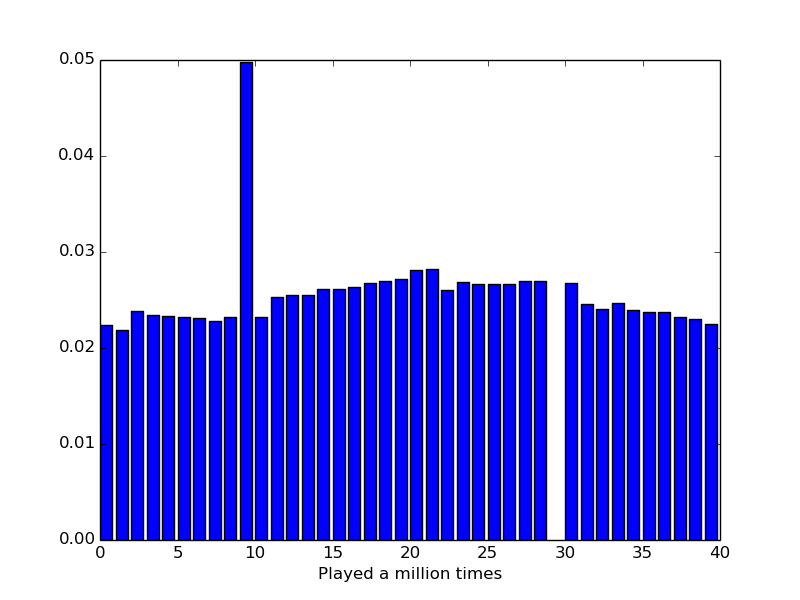
\includegraphics{./monopoly.png}
\caption{A million time of monopoly}
\end{figure}

Although the indexing is somewhat confusing in simulation and Markovian
processing (dropping index 29) altogether. Surprisingly I am getting a
peak at index 21 which is 22 on the board. Markovian process is giving a
peak at index 16 which is definitely somewhat spooky. May be random no
generator mimicking dice is not so great.

\section{Appendix}\label{appendix}

The following code both simulate the game and solves it using stochastic
matrix.

\begin{scriptsize}
    \verbatiminput{./monopoly.py}
\end{scriptsize}

\end{document}
